\graphicspath{
    {figures_and_references/footprints_paper/}
    {figures_and_references/EELISA_conference/}
}

% \selectlanguage{english}
\renewcommand{\chapternametext}{Chapter \thechapter: The \texttt{SeismicBuildingExposure} Python Package}


\chapter{\chapternametext}
\

\renewcommand{\headingtextL}{}
\renewcommand{\headingtextR}{\chapternametext}
\begingroup
 \flushbottom
 \setlength{\parskip}{0pt plus 1fil}%
 \localtableofcontents 
\endgroup

\begingroup
 \flushbottom
 \setlength{\parskip}{0pt plus 1fil}%
 \locallistoffigures
\endgroup


\newpage

\setcounter{section}{0} 



\FloatBarrier

\renewcommand{\sectionnametext}{Introduction}
\renewcommand{\headingtextL}{\chapternametext}
\renewcommand{\headingtextR}{\thesection. \sectionnametext}
\section{\sectionnametext}


The open-source Python package \texttt{SeismicBuildingExposure} has been developed alongside this paper to facilitate the practical application of our research in diverse geographic contexts (available under \url{https://github.com/GeomaticsCaminosUPM/SeismicBuildingExposure/tree/main}). 
Its primary objective is to enable the semi-automatic generation of a comprehensive building exposure inventory at the individual building level, using only geospatial and remote sensing techniques.

In practical terms, the footprint-related workflow involves the following steps: acquiring high-resolution orthoimagery; automatically generating initial building footprint geometries using the Mask2Former model; refining those geometries with the SAM2 model and minimal human intervention; automatically determining the building's direction and relative position within its block; selecting the applicable seismic code; and finally, computing code-relevant geometric parameters automatically and deriving the footprint shape index by applying code-based constraints (fig \ref{fig:workflow}).

\begin{figure}[htbp]
    \centering
    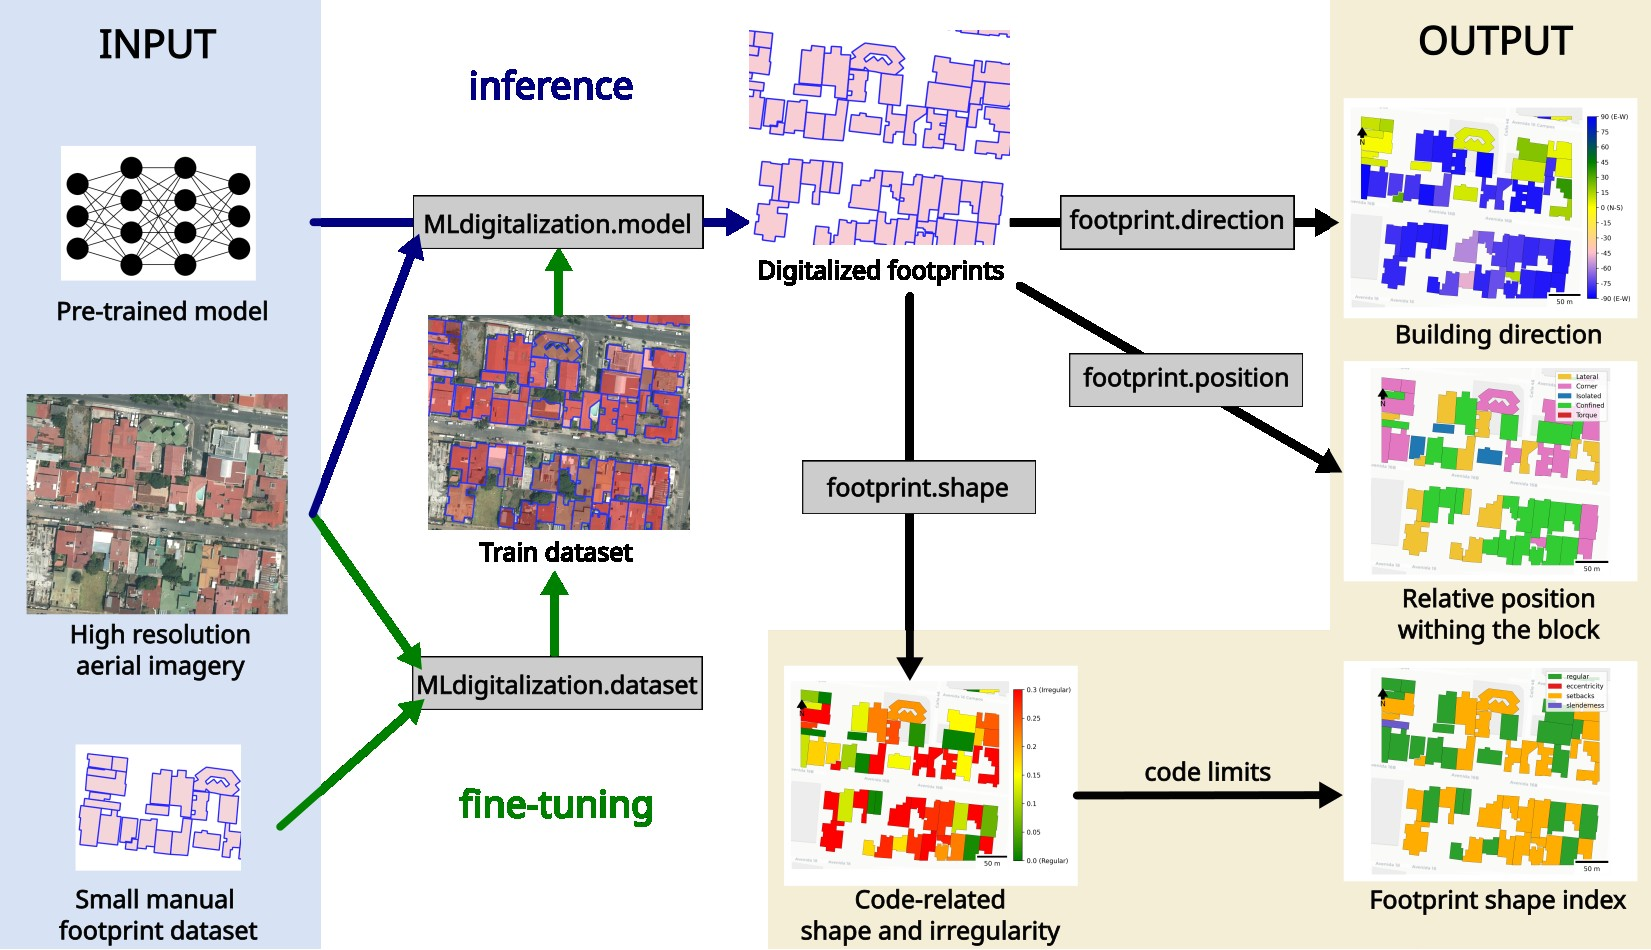
\includegraphics[width=0.85\linewidth]{figures/process.jpg}
    \caption{Semi-automatic seismic exposure inventory generation workflow.}
    \label{fig:workflow}
\end{figure}

\renewcommand{\sectionnametext}{Modules}
\renewcommand{\headingtextL}{\chapternametext}
\renewcommand{\headingtextR}{\thesection. \sectionnametext}
\section{\sectionnametext}

The package is organized into the following submodules:

\begin{itemize}
    \item \textbf{MLdigitalisation.dataset} — Generates computer vision datasets in COCO format from online aerial imagery and a corresponding building footprint geometry file.
    
    \item \textbf{MLdigitalisation.model} — Enables model training on prepared datasets and performs inference on new imagery using pre-trained Mask2Former and SAM2 models to extract building footprint geometries.
    
    \item \textbf{footprint.direction} — Calculates the direction of the building based on the major principal axis of the footprint.
    
    \item \textbf{footprint.position} — Determines the building’s relative position within its urban block.
    
    \item \textbf{footprint.shape} — Computes geometric shape indices in accordance with relevant seismic codes.

    \item \textbf{height} (planned) — Will assess height-related irregularities and vertical configurations.
    
    \item \textbf{remote\_sensing} (planned) — Will include modules for estimating construction year, retrofit status, roof material, and generating digital surface models using remote sensing data.
    
    \item \textbf{MLstructural\_system} — Will offer a machine learning-based classifier to infer structural systems based on geospatial and footprint-derived attributes.
\end{itemize}